\documentclass[12pt,letterpaper]{article}
\usepackage[margin=0.55in,top=0.67in,bottom=0.6in]{geometry}
\usepackage[T1]{fontenc}
\usepackage{helvet}
\renewcommand{\familydefault}{\sfdefault}
\usepackage{tikz}
\usetikzlibrary{arrows.meta}
\usepackage{fancyhdr}
\usepackage{microtype}
\pagestyle{fancy}
\fancyhf{}
\fancyhead[L]{\fontsize{10.5}{12}\selectfont Week 1 / Pattern-block return visits / Grades 2--5}
\fancyfoot[L]{\fontsize{9}{11}\selectfont Bellingham Math Circle / Week 1 / W01-RV-v1}
\fancyfoot[R]{\fontsize{9}{11}\selectfont\thepage}
\renewcommand{\headrulewidth}{0.4pt}
\renewcommand{\footrulewidth}{0pt}
\setlength{\headheight}{15pt}
\setlength{\parindent}{0pt}
\setlength{\parskip}{8pt}
\definecolor{blockgreen}{RGB}{184,218,165}
\definecolor{blockblue}{RGB}{166,205,230}
\tikzset{piece/.style={draw=black,line width=0.8pt,line join=round},
  panel/.style={draw=black!35,line width=0.45pt},
  arrow/.style={-{Stealth[length=2.2mm]},line width=0.8pt}}
\newcommand{\problem}[2]{\textbf{Problem #1:} #2\par}
\newcommand{\gridpanel}[2]{%
  \begin{scope}[shift={(#1,#2)}]
    \draw[panel] (0,0) rectangle (6.81,2.5);
    \begin{scope}
      \clip (0.09,0.35) rectangle (6.72,2.41);
      \foreach \row in {0,...,10} {
        \foreach \col in {0,...,30} {
          \fill[black!18] ({0.12+0.22*\col+0.11*mod(\row,2)},{0.42+0.190526*\row}) circle (0.007);
        }
      }
    \end{scope}
    \node[anchor=west,font=\fontsize{10}{12}\selectfont] at (0.12,0.17) {Boundary: \rule{0.45in}{0.4pt}\ block sides};
  \end{scope}%
}
\newcommand{\cornerpanel}[2]{%
  \begin{scope}[shift={(#1,#2)}]
    \draw[panel] (0,0) rectangle (3.28,1.35);
    \fill (1.64,0.86) circle (0.022);
    \node[anchor=west,font=\fontsize{10}{12}\selectfont] at (0.12,0.16) {Triangles: \rule{0.3in}{0.4pt}\quad Rhombi: \rule{0.3in}{0.4pt}};
  \end{scope}%
}
\newcommand{\hexrecord}[2]{%
  \begin{scope}[shift={(#1,#2)}]
    \draw[panel] (0,0) rectangle (3.28,2.15);
    \begin{scope}[shift={(1.64,1.24)}]
      \draw[line width=0.85pt] (0:0.83) \foreach \a in {60,120,180,240,300} {-- (\a:0.83)} -- cycle;
    \end{scope}
    \node[anchor=west,font=\fontsize{10}{12}\selectfont] at (0.12,0.25) {Matching turns (steps):};
    \foreach \n in {1,...,5} {
      \node[font=\fontsize{12}{14}\selectfont] at ({1.58+0.3*\n},0.25) {\n};
    }
  \end{scope}%
}
\begin{document}
\fontsize{13.5}{18}\selectfont
Use small green triangles, small blue rhombi, or both. Pieces must not overlap.

\problem{1}{Use exactly 6 green triangles and 2 blue rhombi. Join all eight blocks into one shape along whole sides. Make a shape with the shortest boundary you can, and one with the longest. Count the uncovered block sides, including any around a hole, and sketch both shapes.}

\vspace{2pt}
\begin{center}
\begin{tikzpicture}[x=1in,y=1in]
  \gridpanel{0}{2.75}
  \gridpanel{0}{0}
\end{tikzpicture}
\end{center}
\newpage

\problem{2}{On the table, build as many different arrangements as you can that close around one point with no gaps. Every piece must have a corner at the point. A new arrangement must use different numbers of triangles or rhombi. Sketch each successful arrangement and write its two counts.}

\begin{center}
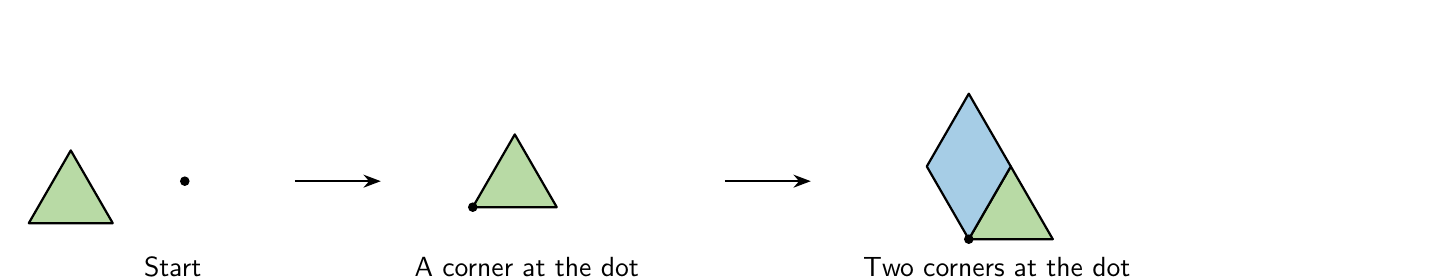
\begin{tikzpicture}[x=1in,y=1in]
  \begin{scope}[shift={(0.35,0.12)},scale=0.6]
    \fill (0.55,0.35) circle (0.04);
    \draw[piece,fill=blockgreen] (-0.75,0) -- (-0.05,0) -- (-0.4,0.606218) -- cycle;
  \end{scope}
  \node[font=\fontsize{10}{12}\selectfont] at (0.62,-0.1) {Start};
  \draw[arrow] (1.23,0.33) -- (1.66,0.33);
  \begin{scope}[shift={(2.12,0.2)},scale=0.6]
    \draw[piece,fill=blockgreen] (0,0) -- (0.7,0) -- (0.35,0.606218) -- cycle;
    \fill (0,0) circle (0.04);
  \end{scope}
  \node[font=\fontsize{10}{12}\selectfont] at (2.39,-0.1) {A corner at the dot};
  \draw[arrow] (3.38,0.33) -- (3.81,0.33);
  \begin{scope}[shift={(4.6,0.04)},scale=0.6]
    \draw[piece,fill=blockgreen] (0,0) -- (0.7,0) -- (0.35,0.606218) -- cycle;
    \draw[piece,fill=blockblue] (0,0) -- (0.35,0.606218) -- (0,1.212436) -- (-0.35,0.606218) -- cycle;
    \fill (0,0) circle (0.04);
  \end{scope}
  \node[font=\fontsize{10}{12}\selectfont] at (4.74,-0.1) {Two corners at the dot};
  \path (0,-0.22) rectangle (6.81,0.89);
\end{tikzpicture}
\end{center}
\vspace{-2pt}
\begin{center}
\begin{tikzpicture}[x=1in,y=1in]
  \cornerpanel{0}{4.35}
  \cornerpanel{3.53}{4.35}
  \cornerpanel{0}{2.90}
  \cornerpanel{3.53}{2.90}
  \cornerpanel{0}{1.45}
  \cornerpanel{3.53}{1.45}
  \cornerpanel{0}{0}
  \cornerpanel{3.53}{0}
\end{tikzpicture}
\end{center}
\newpage

A 1-step turn moves each corner clockwise to the next corner. The blocks and their inside edges turn together.
\begin{center}
\begin{tikzpicture}[x=1in,y=1in]
  \begin{scope}[shift={(0.79,0.55)}]
    \draw[line width=0.75pt] (0:0.43) \foreach \a in {60,120,180,240,300} {-- (\a:0.43)} -- cycle;
    \fill (60:0.43) circle (0.045);
  \end{scope}
  \node[font=\fontsize{10}{12}\selectfont] at (0.79,-0.03) {Start};
  \draw[arrow] (1.54,0.55) -- (1.96,0.55);
  \begin{scope}[shift={(2.77,0.55)}]
    \draw[black!50,line width=0.75pt] (0:0.43) \foreach \a in {60,120,180,240,300} {-- (\a:0.43)} -- cycle;
    \draw[arrow] (62:0.57) arc[start angle=62,end angle=0,radius=0.57];
    \draw[black!50,line width=0.65pt] (60:0.43) circle (0.045);
  \end{scope}
  \node[font=\fontsize{10}{12}\selectfont] at (2.77,-0.03) {Turn 1 step};
  \draw[arrow] (3.52,0.55) -- (3.94,0.55);
  \begin{scope}[shift={(4.75,0.55)}]
    \draw[line width=0.75pt] (0:0.43) \foreach \a in {60,120,180,240,300} {-- (\a:0.43)} -- cycle;
    \fill (0:0.43) circle (0.045);
  \end{scope}
  \node[font=\fontsize{10}{12}\selectfont] at (4.75,-0.03) {After};
  \path (0,-0.15) rectangle (6.81,1.13);
\end{tikzpicture}
\end{center}
\vspace{-3pt}
\problem{3}{On the table, fill a regular hexagon with these blocks. Its outer sides are each one block side. Which turns make your design match itself, including every edge inside? Make designs with different answers. Sketch each design and circle every turn that works.}

\begin{center}
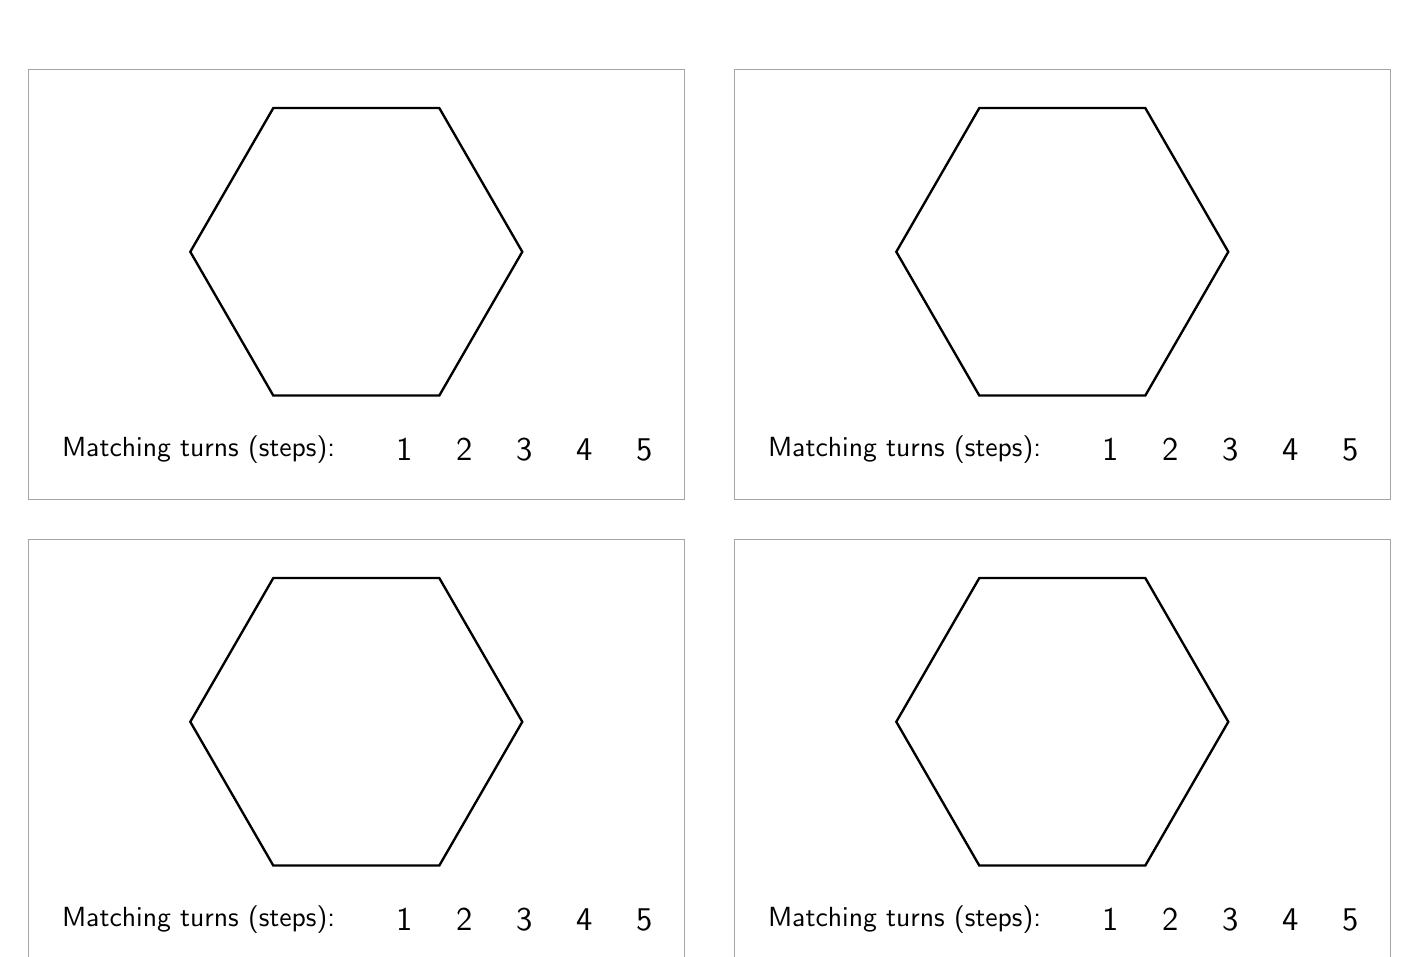
\begin{tikzpicture}[x=1in,y=1in]
  \hexrecord{0}{2.35}
  \hexrecord{3.53}{2.35}
  \hexrecord{0}{0}
  \hexrecord{3.53}{0}
\end{tikzpicture}
\end{center}
\end{document}
